\documentclass[a4paper, UKenglish]{article}
%% Encoding
\usepackage[utf8]{inputenx}
\usepackage[T1]{fontenc}

%% Fonts and typography
\usepackage{lmodern}           % Latin Modern Roman
\usepackage[scaled]{beramono}  % Bera Mono (Bitstream Vera Sans Mono)
\renewcommand{\sfdefault}{phv} % Helvetica
\usepackage[bf, sf]{titlesec}  % Section headings
\usepackage[final]{microtype}  % Improved typography


%% Mathematics
\usepackage{amssymb}   % Extra symbols
\usepackage{amsthm}    % Theorem-like environments
\usepackage{thmtools}  % Theorem-like environments
\usepackage{mathtools} % Fonts and environments for mathematical formuale
\usepackage{mathrsfs}  % Script font with \mathscr{}
\usepackage{amsmath}


%% Miscellanous
\usepackage{graphicx}   	% Tool for images
\usepackage{subcaption} 	% Tool for images
\usepackage[UKenglish]{babel}   % Automatic translations
\usepackage{csquotes}   	% Quotes
\usepackage{textcomp}   	% Extra symbols
\usepackage{booktabs}   	% Tool for tables
\usepackage{float}

\usepackage[usenames,dvipsnames]{xcolor}
\definecolor{lbcolor}{rgb}{0.9,0.9,0.9}
\usepackage{listings}   % Typesetting code
%\lstset{backgroundcolor=\color{lbcolor}, basicstyle = \ttfamily, frame = %single, language=python}
\lstset{
	backgroundcolor=\color{lbcolor},
	tabsize=4,
	rulecolor=,
	language=java,
        basicstyle=\scriptsize,
        upquote=true,
        aboveskip={1.5\baselineskip},
        columns=fixed,
	numbers=left,
        showstringspaces=false,
        extendedchars=true,
        breaklines=true,
        prebreak = \raisebox{0ex}[0ex][0ex]{\ensuremath{\hookleftarrow}},
        frame=single,
        showtabs=false,
        showspaces=false,
        showstringspaces=false,
        identifierstyle=\ttfamily,
        keywordstyle=\color[rgb]{0,0,1},
        commentstyle=\color[rgb]{0.133,0.545,0.133},
        stringstyle=\color[rgb]{0.627,0.126,0.941}
        }

%% Bibliography
%\usepackage[backend = biber, style = alphabetic]{biblatex}
%\addbibresource{<NAME OF BIBLIOGRAPY FILE>.bib}


%% Cross references
\usepackage{varioref}
\usepackage{hyperref}
\urlstyle{sf}
\usepackage[nameinlink, capitalize, noabbrev]{cleveref}


%% Theorem-like environments
\declaretheorem[style = plain, numberwithin = section]{theorem}
\declaretheorem[style = plain,      sibling = theorem]{corollary}
\declaretheorem[style = plain,      sibling = theorem]{lemma}
\declaretheorem[style = plain,      sibling = theorem]{proposition}
\declaretheorem[style = definition, sibling = theorem]{definition}
\declaretheorem[style = definition, sibling = theorem]{example}
\declaretheorem[style = remark,    numbered = no]{remark}


%% Delimiters
\DeclarePairedDelimiter{\p}{\lparen}{\rparen}   % Parenthesis
\DeclarePairedDelimiter{\set}{\lbrace}{\rbrace} % Set
\DeclarePairedDelimiter{\abs}{\lvert}{\rvert}   % Absolute value
\DeclarePairedDelimiter{\norm}{\lVert}{\rVert}  % Norm


%% Operators
\DeclareMathOperator{\im}{im}
\DeclareMathOperator{\rank}{rank}
\DeclareMathOperator{\E}{E}
\DeclareMathOperator{\Var}{Var}
\DeclareMathOperator{\Cov}{Cov}


%% New commands for sets
\newcommand{\N}{\mathbb{N}}   % Natural numbers
\newcommand{\Z}{\mathbb{Z}}   % Integers
\newcommand{\Q}{\mathbb{Q}}   % Rational numbers
\newcommand{\R}{\mathbb{R}}   % Real numbers
\newcommand{\C}{\mathbb{C}}   % Complex numbers
\newcommand{\A}{\mathbb{A}}   % Affine space
\renewcommand{\P}{\mathbb{P}} % Projective space


%% New commands for vectors
\renewcommand{\a}{\mathbf{a}}
\renewcommand{\b}{\mathbf{b}}
\renewcommand{\c}{\mathbf{c}}
\renewcommand{\v}{\mathbf{v}}
\newcommand{\w}{\mathbf{w}}
\newcommand{\x}{\mathbf{x}}
\newcommand{\y}{\mathbf{y}}
\newcommand{\z}{\mathbf{z}}
\newcommand{\0}{\mathbf{0}}
\newcommand{\1}{\mathbf{1}}


%% Miscellanous
\renewcommand{\qedsymbol}{\(\blacksquare\)}


%% Things I've put in meself
\usepackage{tikz}
\usetikzlibrary{decorations.pathreplacing,angles,quotes}
\newcommand*\circled[1]{\tikz[baseline=(char.base)]{
            \node[shape=circle,draw,inner sep=2pt] (char) {#1};}}
\usepackage{arydshln}
\newcommand{\citesup}[1]{\textsuperscript{\cite{#1}}}



\begin{document}
\title{FYS-STK 3155 project 3: A Study of Heart Failure}
\author{Theodor Midtbø Alstad}
\maketitle

\begin{abstract}
This report analyzes a dataset on heart failure published by user Larxel on Kaggle, using a custom Logistic Regressor, a custom Neural Network, a Random Forest from scikit-learn, and a custom Ridge regressor. It finds that scikit-learns Random Forest has the highest rate of accuracy, and that the Logistic Regressor has the highest rate of positives detected.
\end{abstract}




\section{Introduction}
Cardiovascular diseases are the leading causes of death in the world\citesup{top10death}, and understanding their causes can help efforts in combating death. 

This report discusses a dataset regarding heart failure\citesup{dataset}, building on theory from previous projects\citesup{project_1}\citesup{project_2}. This dataset contains 12 features, one of which is a response variable, and 299 datapoints.

In this project, I analyze the aforementioned dataset using 4 different methods, with the intent of finding the best algorithm for this dataset: ScikitLearns Random Forest, Logistic Regression, Neural Network, and Ridge linear regression.

Structurally, this report:
\begin{itemize}
\item1: Builds on theory previously described in an earlier project\citesup{project_2}.
\item2: Describing the dataset used.
\item3: Referencing other literature.
\item4: Describing what algorithms were used and what distinguishes them.
\item5: Providing the results found.
\item6: Discussing the results and finding conclusions.
\end{itemize} 

\section{Theory}
I am using algorithms developed in a previous project\citesup{project_2}, where the theory of Ridge, basic SGD, momentum, minibatching, varying step length, and $l_2$ regularization parameters is described, so I will refer to that, but will extend the theory on Neural Network and Logistic Regression.

\subsection{Confusion matrix}
When using a binary classification algorithm, you could either get a correct answer or an incorrect answer. This could be further detailed by describing in what way the classification is correct or incorrect, by describing whether the algorithm is correct or incorrect and what option it chose. You can describe this detail using a confusion matrix:

\begin{table}[H]
\centering
\caption{An example confusion matrix}
\label{tab:confusion matrix}
\begin{tabular}{|c||c|c|}
    \hline
           & Positive   & Negative   \\
\hline
\hline
    Pred. Positive & True Positive  & False Positive \\
    \hline
    Pred. Negative & False Negative & True Negative  \\
    \hline
\end{tabular}
\end{table}



\subsection{Logistic Regression}
Building on the theory described in my previous report\citesup{project_2}, this section goes into more detail on the actual algorithm of my Logistic Regressor.

\subsubsection{Prediction}
A Logistic Regressor takes a set of datapoints, $\textbf{X}$, and uses a set of weights, $\theta$, in a matrix multiplication $\mathbf{X} \times \theta = \textbf{z}$ with the shape $\left(1\times p\right) \times \left(p\times k\right) = \left(k\times1\right)$. Since this is a matrix multiplication $\mathbf{X}$ can be expanded to contain multiple sets of datapoints, $\mathbf{X} \in  \mathbb{R}^{n\times p}$ to make multiple predictions at once without changing the weights. The resulting $z$ is finally put through an output function, here Softmax, giving a final prediction.: $$\text{softMax}(z) = \frac{e^z}{\sum\limits_{i=0}^{k-1}\left(z_i\right)}$$

\subsubsection{Correction/Backpropagation}
The first time a Logistic Regressor is used $\theta$ is somehow initialized to a set of values, here randomly uniformly distributed between 0 and 1. The first prediction a Logistic Regressor makes is likely to be very wrong due to the random weights, and this is where the training process starts. When the regressor makes a prediction, it is compared to set of values that is known to be the correct prediction for the given datapoints, $\bar{z}$, and an error is generated by using the appropriate cost function, here simply being the difference between the two: $C(z) = z - \bar{z}$. This error is then applied to the weights through matrix multiplication, $\theta \leftarrow \theta - \textbf{X}^T \times C(z)$. This prediction-and-correction cycle is repeated for a number of sets of data, repeatedly training the regressor, becoming more and more accurate.


\subsection{Neural Network}
A Neural Network functions like an extension to the Logistic Regressor, where there are layers, called hidden layers, put between the input and the output layers. The network makes predictions, much like the Logistic Regressor, by multiplying the input, $\textbf{X}$ by a set of weights and putting the result through an activation function (sigmoid, ReLU, etc.), except that for the network, this result is multiplied by another set of weights and put through the activation function again, repeating for each hidden layer (creating what is known as activation values, $a_{ln}$ for a single node or $a_l$ for an entire layer, the output of a node in a layer that is to be put through the activation function, where $a_0 = \textbf{X}$) until an output is generated; for a network with $l=3$ hidden layers, it would function as $((((\textbf{X}\times \theta_0)\times \theta_1)\times \theta_2)\times \theta_f) = \textbf{X}\times\prod\limits^2_{i=0} (\theta_i) \times \theta_f = z$. Similarly to the Logistic Regressor, an error-value is generated, $\epsilon = z - \bar{z}$, and is backpropagated through the network in a similar, if more convoluted, way; $\theta_i \leftarrow \theta_i - (\epsilon\times\theta_f f'(a_{l})) \times (\theta_{l-1}f'(a_{l-1})) \times (\theta_{l-2}f'(a_{l-2})) ... \times (\theta_if'(a_{i}))\times f(a_i)$, where f() is the activation function.

The fact that the same error is multiplied throughout the network can lead to issues where the gradient, how much the weights change, vanishes or explodes as it is calculated further down the network, but the details if this occurrence is not within the scope of this report.

Each node can use a different activation function, and each layer could have a different number of nodes, but in the case of the network used in this report, each layer has the same number of nodes, and all nodes use the same activation function (sigmoid, which was found through a grid search to give optimal results) except for the final ones (using the softMax function).

\subsection{Random Forest}
\subsubsection{Decision Trees}
Since the structure of a Random Forest relies heavily on the structure of a decision tree, it is only natural to describe it first.

A decision tree tries to predict data by separating it into several binary or discretized decisions, splitting into a sub-tree for each possible decision, repeating this process until it comes to a "leaf", where the training algorithm has decided on a prediction. A relevant example could be the algorithm asking whether the patient smokes, going to the sub-tree for "no" if the patient doesn't smoke, then asking whether the ejection\_fraction is above or below 0.4, going to the relevant sub-tree, finally asking whether the patient has diabetes, and reaching a decision on DEATH\_EVENT from this. Of note is that any continuous feature has to be discretized to fit into a decisions tree, usually by defining ranges and creating sub-trees based on what range the relevant feature is in (as was shown in the relevant example).

A decision tree is very simple to implement, use, and interpret, is good at predicting, but is very prone to overfitting\citesup{Flom_2019}. 

\subsubsection{Reducing Overfitting}
In order to reduce overfitting in decision trees, they are organized into structures called Random Forests, which contains multiple decision trees, but each decision tree is constructed from a bootstrapped\citesup{project_1} version of the dataset, and estimating a prediction based on the prediction in each component decision tree.


\subsection{Other literature}
Sakhiya, Nayan\citesup{nayan} graphically describes each individual feature in terms of its correlation to DEATH\_EVENT and decides to model the data using the features "time", "ejection\_fraction", and "serum\_creatinine" and manages to get an accuracy of up to 93.33\% with a Gradient Booster Classifier and 90.00\% with a Random Forest Classifier and Logistic Regressor. They do, however, inadvisably use the time feature and use a random state in their train-test data split that, according to a commenter named BloodCoder16, would lead to an accuracy of 85\% with other random states. Whilst this leads to doubt about the useability of the predictions themselves, the individual features are well analyzed.

\section{Dataset}
The dataset used\citesup{dataset} deals with heart failure as a binary classification problem. There are 12 input data and 1 response datum. It was published by the user Larxel on Kaggle June 2020. 6 of the features are discrete and 6 are continuous. The data is scaled by dividing each feature by the average value of that feature.

\subsection{Features}


\begin{table}[H]
\centering
\caption{Input features}
\label{tab:input features}
\begin{tabular}{|l|l||l|}
    \hline
    Feature & Description & (datatype) [Unit] \\
    \hline
    \hline
    Age & Age of the patient & (float) [years] \\
    \hline
    Anaemia & Whether the patient is anaemic & (boolean) [true/false] \\
    \hline
    Creatinine & Level of the CPK enzyme in the &(float) [mcg/L]  \\
    Phosphokinase &patients blood &  \\
    \hline
    Diabetes & Whether the patient was diabetic & (boolean) [true/false] \\
    \hline
    Ejection Fraction & Percentage of blood in heart being  & (percentage) [\%]  \\&pumped out at each contraction & \\
    \hline
    High Blood Pressure & Whether the patient has hypertension &(boolean) [true/false] \\
    \hline
    Platelets & Level of platelets in the blood &(float) [kiloplatelets/mL] \\
    \hline
    Serum Creatinine & Level of serum creatinine &(float) [mg/dL] \\ & in the blood &  \\
    \hline
    Serum Sodium & Level of serum sodium in the blood &(float) [mEq/L] \\
    \hline
    Sex & Whether the patient is male of female &(binary) [male/female] \\
    \hline
    Smoking &  Whether the patient smokes &(boolean) [true/false] \\
    \hline
    \hline
    Time & The duration of the study  & (integer) [days] \\
    &on the subject &\\
    \hline
\end{tabular}
\end{table}

The time feature is the amount of time the study went on for and is ignored here because it is only gained at the end of the study and can thus not only only be known ahead of time and is not useable as a predictor, but also has a strong correlation to DEATH\_EVENT, and will artificially inflate accuracy.

The sex feature is given as binary, but will be treated as a boolean (using the already binary 0 and 1 as false and true, respectively) for ease of implementation.

\begin{table}[H]
\centering
\caption{Response features}
\label{tab:response features}
\begin{tabular}{|l|l||l|}
    \hline
    Feature & Description & (datatype) [Unit] \\
    \hline
    \hline
    DEATH\_EVENT & Whether the subject died during the study& (boolean) [true/false] \\
    \hline
\end{tabular}
\end{table}

A negative response variable indicates that the study terminated without the subject dying. It is assumed that this means that the subject was written off as healthy and does not pose a risk of dying of heart disease.

\section{Methods}
4 algorithms were tested on this dataset, 3 of which were custom-made (Random Forest was imported from sklearn\citesup{sklearn}, included to include professionally constructed algorithms) and 3 of which is traditionally used for classification (Ridge is typically used for regression on continuous response variables, included to include non-traditional methods). They were all evaluated using a grid search to find optimal parameters


\section{Results}

\subsection{Features}
Features represented using tables and histograms to show their individual correlation to DEATH\_EVENT. The tables include an extra row showing survival rate for each possibility. The histograms have been normalized for a total area of 1 for ease of comparison. A higher DEATH\_EVENT False divided by DEATH\_event True, i.e. a higher survival rate, is better.

\begin{table}[H]
\centering
\caption{Table of correlation between boolean anaemia and DEATH\_EVENT}
\label{tab:anaemia}
\begin{tabular}{|c||c|c|}
    \hline
       & anaemia True   & anaemia False   \\
    \hline
    \hline
    DEATH{\_}EVENT True & 46.00  & 50.00 \\
    \hline
    DEATH{\_}EVENT False & 83.00 & 120.00  \\
    \hline
    \hline
    DEATH{\_}EVENT False & & \\
    divided by & 1.80 & 2.40 \\
    DEATH{\_}EVENT True & & \\
    \hline
\end{tabular}
\end{table}


\begin{table}[H]
\centering
\caption{Table of correlation between boolean diabetes and DEATH\_EVENT}
\label{tab:diabetes}
\begin{tabular}{|c||c|c|}
    \hline
       & diabetes True   & diabetes False   \\
    \hline
    \hline
    DEATH{\_}EVENT True & 40.00  & 56.00 \\
    \hline
    DEATH{\_}EVENT False & 85.00 & 118.00  \\
    \hline
    \hline
    DEATH{\_}EVENT False & & \\
    divided by & 2.12 & 2.11 \\
    DEATH{\_}EVENT True & & \\
    \hline
\end{tabular}
\end{table}


\begin{table}[H]
\centering
\caption{Table of correlation between boolean high{\_}blood{\_}pressure and DEATH\_EVENT}
\label{tab:high_blood_pressure}
\begin{tabular}{|c||c|c|}
    \hline
       & high{\_}blood{\_}pressure True   & high{\_}blood{\_}pressure False   \\
    \hline
    \hline
    DEATH{\_}EVENT True & 39.00  & 57.00 \\
    \hline
    DEATH{\_}EVENT False & 66.00 & 137.00  \\
    \hline
    \hline
    DEATH{\_}EVENT False & & \\
    divided by & 1.69 & 2.40 \\
    DEATH{\_}EVENT True & & \\
    \hline
\end{tabular}
\end{table}


\begin{table}[H]
\centering
\caption{Table of correlation between boolean sex and DEATH\_EVENT}
\label{tab:sex}
\begin{tabular}{|c||c|c|}
    \hline
       & sex True   & sex False   \\
    \hline
    \hline
    DEATH{\_}EVENT True & 62.00  & 34.00 \\
    \hline
    DEATH{\_}EVENT False & 132.00 & 71.00  \\
    \hline
    \hline
    DEATH{\_}EVENT False & & \\
    divided by & 2.13 & 2.09 \\
    DEATH{\_}EVENT True & & \\
    \hline
\end{tabular}
\end{table}


\begin{table}[H]
\centering
\caption{Table of correlation between boolean smoking and DEATH\_EVENT}
\label{tab:smoking}
\begin{tabular}{|c||c|c|}
    \hline
       & smoking True   & smoking False   \\
    \hline
    \hline
    DEATH{\_}EVENT True & 30.00  & 66.00 \\
    \hline
    DEATH{\_}EVENT False & 66.00 & 137.00  \\
    \hline
    \hline
    DEATH{\_}EVENT False & & \\
    divided by & 2.20 & 2.08 \\
    DEATH{\_}EVENT True & & \\
    \hline
\end{tabular}
\end{table}

\begin{table}[H]
\centering
\caption{Table of correlation between boolean DEATH{\_}EVENT and DEATH\_EVENT. This is included for completeness}
\label{tab:DEATH_EVENT}
\begin{tabular}{|c||c|c|}
    \hline
       & DEATH\_EVENT True   & DEATH\_EVENT False   \\
    \hline
    \hline
    DEATH{\_}EVENT True & 96.00  & 0.00 \\
    \hline
    DEATH{\_}EVENT False & 0.00 & 203.00  \\
    \hline
\end{tabular}
\end{table}

From the tables, the two features that stand out as having a larger individual impact are high blood pressure and anaemia with a decreased survival rate of 29.58\% and 25.00\%, respectively, followed by smoking and sex, increasing survival rate by 5.77\% and  1.91\%. respectively.


\begin{figure}[H]
        \centering
        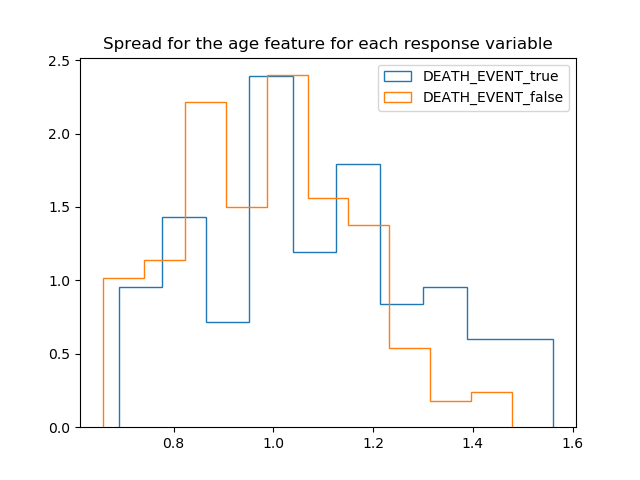
\includegraphics[scale=0.6]{images/age.png}
        \caption{Histogram presenting the age feature for DEATH{\_}EVENT being True and False}
        \label{fig:age}
\end{figure}


\begin{figure}[H]
        \centering
        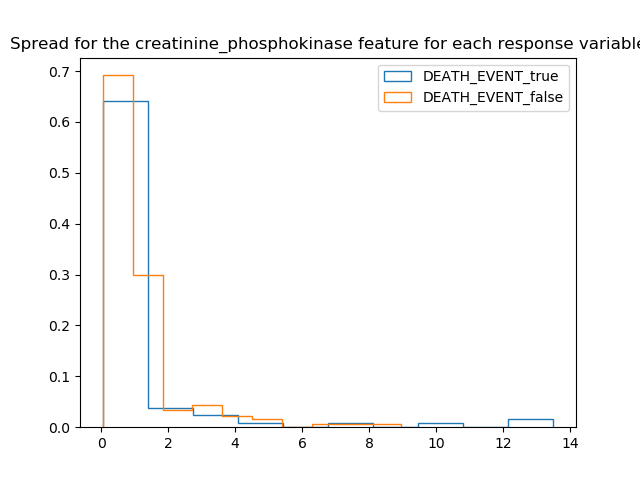
\includegraphics[scale=0.6]{images/creatinine_phosphokinase.png}
        \caption{Histogram presenting the creatinine{\_}phosphokinase feature for DEATH{\_}EVENT being True and False}
        \label{fig:creatinine_phosphokinase}
\end{figure}


\begin{figure}[H]
        \centering
        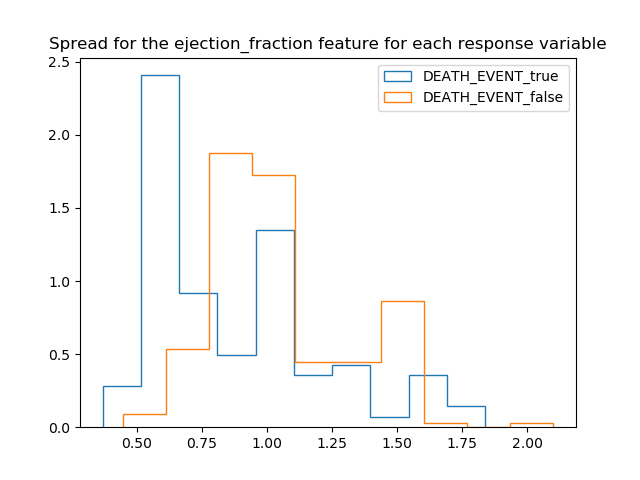
\includegraphics[scale=0.6]{images/ejection_fraction.png}
        \caption{Histogram presenting the ejection{\_}fraction feature for DEATH{\_}EVENT being True and False}
        \label{fig:ejection_fraction}
\end{figure}


\begin{figure}[H]
        \centering
        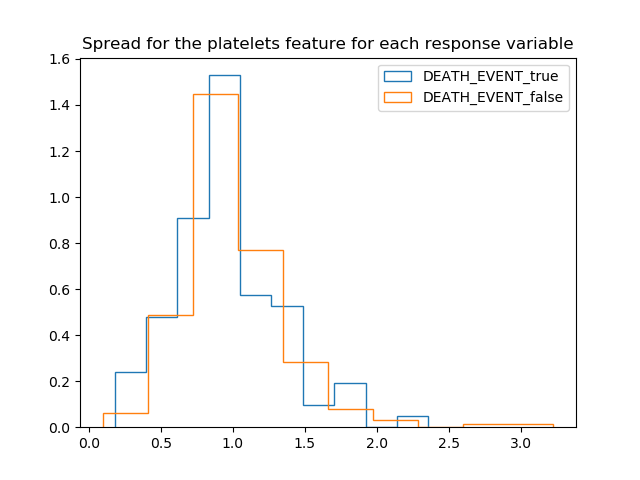
\includegraphics[scale=0.6]{images/platelets.png}
        \caption{Histogram presenting the platelets feature for DEATH{\_}EVENT being True and False}
        \label{fig:platelets}
\end{figure}


\begin{figure}[H]
        \centering
        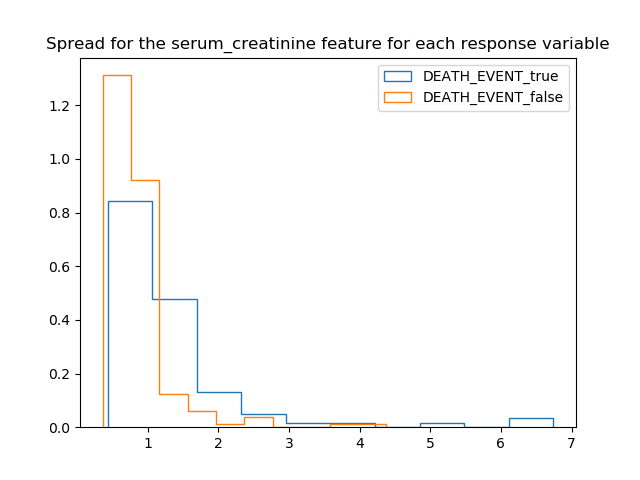
\includegraphics[scale=0.6]{images/serum_creatinine.png}
        \caption{Histogram presenting the serum{\_}creatinine feature for DEATH{\_}EVENT being True and False}
        \label{fig:serum_creatinine}
\end{figure}


\begin{figure}[H]
        \centering
        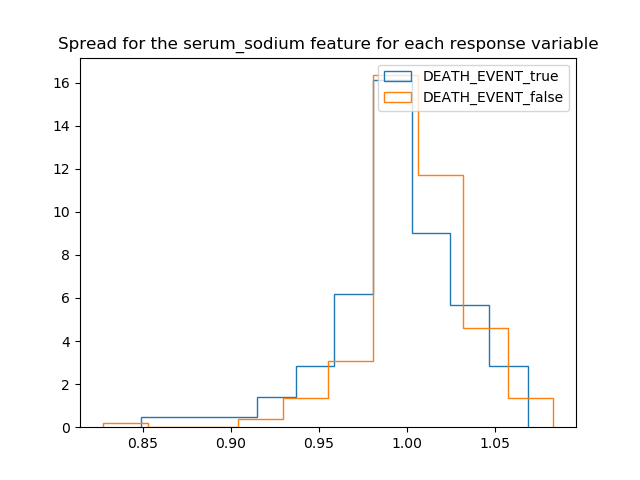
\includegraphics[scale=0.6]{images/serum_sodium.png}
        \caption{Histogram presenting the serum{\_}sodium feature for DEATH{\_}EVENT being True and False}
        \label{fig:serum_sodium}
\end{figure}


Given time constraints, the histogram correlations will not be numerically analyzed, but I will refer to N. Sakhiya\citesup{nayan} choosing ejection\_fraction and serum\_creatinine as strong predictors.


\subsection{Prediction power}
All confusion matrices generated as an average over 1000 different train/test splits and trainings. The confusion matrices are generated from the testing samples and thus contain $ceil(299/4) = 75$ total samples.


\begin{table}[H]
\centering
\caption{Confusion table for Neural Network as an average over 1000 runs, with an overall accuracy score of 70.07{\%}}
\label{tab:Neural Network}
\begin{tabular}{|c||c|c|}
\hline
Neural Network       & Positive   & Negative   \\
\hline
\hline
Pred. Positive & 8.13  & 6.45 \\
\hline
Pred. Negative & 15.99 & 44.42  \\
\hline
\hline
Rate of Detection & 0.34 & 0.87 \\
\hline
\end{tabular}
\end{table}


\begin{table}[H]
\centering
\caption{Confusion table for Random Forest as an average over 1000 runs, with an overall accuracy score of 73.50{\%}}
\label{tab:Random Forest}
\begin{tabular}{|c||c|c|}
\hline
Random Forest       & Positive   & Negative   \\
\hline
\hline
Pred. Positive & 9.96  & 5.79 \\
\hline
Pred. Negative & 14.08 & 45.17  \\
\hline
\hline
Rate of Detection & 0.42 & 0.89 \\
\hline
\end{tabular}
\end{table}


\begin{table}[H]
\centering
\caption{Confusion table for Ridge as an average over 1000 runs, with an overall accuracy score of 73.14{\%}}
\label{tab:Ridge}
\begin{tabular}{|c||c|c|}
\hline
Ridge       & Positive   & Negative   \\
\hline
\hline
Pred. Positive & 9.50  & 5.43 \\
\hline
Pred. Negative & 14.71 & 45.35  \\
\hline
\hline
Rate of Detection & 0.40 & 0.89 \\
\hline
\end{tabular}
\end{table}


\begin{table}[H]
\centering
\caption{Confusion table for Logistic Classifier as an average over 1000 runs, with an overall accuracy score of 73.42{\%}}
\label{tab:Logistic Classifier}
\begin{tabular}{|c||c|c|}
\hline
Logistic Classifier       & Positive   & Negative   \\
\hline
\hline
Pred. Positive & 10.71  & 6.57 \\
\hline
Pred. Negative & 13.37 & 44.36  \\
\hline
\hline
Rate of Detection & 0.45 & 0.87 \\
\hline
\end{tabular}
\end{table}

\section{Discussion}
Looking at the predictive power of each algorithm, All but the Neural Network perform equally well an overall classifier. Surprisingly enough, I implemented Ridge as an attempt to demonstrate that it is an algorithm traditionally used to regress on continuous values and did not expect it to perform on par with other methods. As an overall predictor, one could pick any one of Random Forest, Ridge, and Logistic Classifier, but given the nature of the dataset, in that it deals with heart failure, weight should be put on minimizing false negatives or maximizing rate of positive detection, which the Logistic Classifier seems to do the best, at 45\% detection rate compared to the closest Random Forest, performing at a 42\% detection rate.

\section{Conclusion}
In this report I have analyzed a dataset on heart failure, looked into the predictive power of individual features, looked at overall predictive power and predictive power for certain modes of the response variable DEATH\_EVENT. I found that scikit-learns Random Forest has the most overall accurate predictions, but not significantly more accurate than Ridge and the Logistic Classifier, and I found that the Logistic Classifier has the highest rate of positive detections (i.e. the lowest rate of false negatives compared to true positives).

\subsection{Considerations for improvements}
This report includes training on all features, even though several have been demonstrated to have much higher predictive power and feature selection, like seen done by N. Sakhiya\citesup{nayan}, could be beneficial. Unfortunately, there has not been enough time to make use of the analysis on the individual impacts from each feature.

Given the nature of this dataset, and how false positives are preferable over false negatives, the regressions could have benefited from changed threshold  in prediction, so that not just the most likely outcome was predicted, but rather positives had a bias so that the false positives detection could with benefit be artificially inflated.



\newpage

\bibliographystyle{ieeetr}
\bibliography{references}


\end{document}